\section{Examples of Instances - Drawings}

\begin{figure}[H]
    \centering
    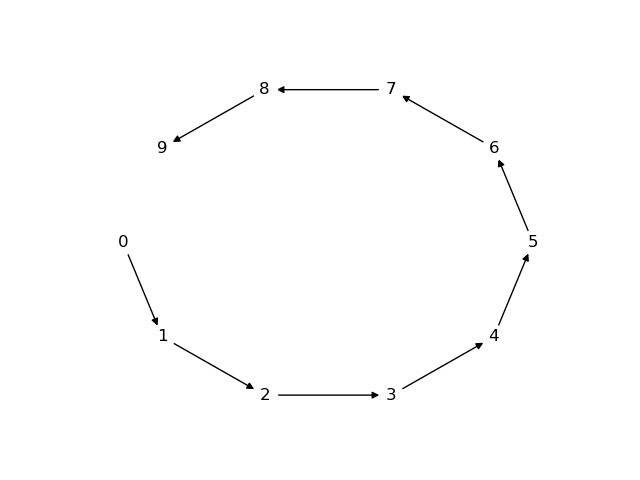
\includegraphics[width=0.4\textwidth]{images/instances_examples/too_easy.png}
    \caption{Example of an instance too easy to solve, the vertices are too tight to one another.}
\end{figure}

\begin{figure}[H]
    \centering
    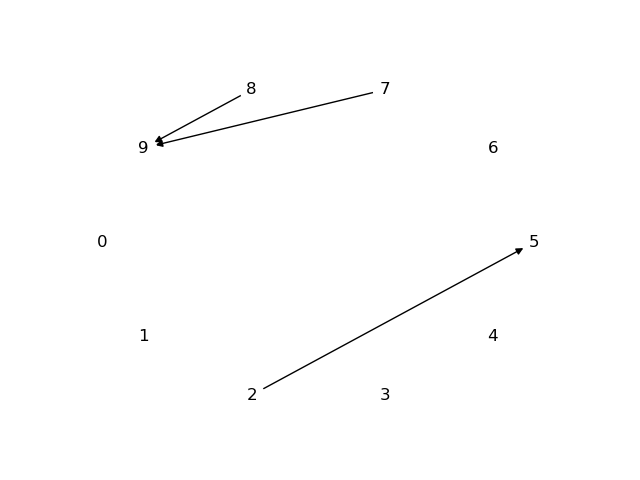
\includegraphics[width=0.4\textwidth]{images/instances_examples/too_difficult.png}
    \caption{Example of an instance too difficult to solve, the vertices are too loose from one another.}
\end{figure}

\begin{figure}[H]
    \centering
    \includegraphics[width=0.4\textwidth]{images/instances_examples/good.png}
    \caption{Example of a good instance, not too hard, not too easy. The vertices are somewhat tight to one another, but not too much.}
\end{figure}
